% Uživatelským požadavkem je dynamické zařízení sloužící například jako identifikátor hráče, nebo jako herní nástroj.
% Mělo by ale být schopno zastat i~roli statického zařízení, pro případy her na delších výletech, kde by bylo nepraktické nosit s~sebou velké zařízení.
% Vyžaduje tedy dostatečnou mobilitu, aby uživateli nepřekáželo v~pohybu.
% Zároveň by zařízení mělo být co nejlevnější pro možnost nasazení ve velkém počtu.
% Z~toho plynou požadavky na výslednou konstrukci a velikost zařízení.

% Zařízení by mělo být schopno komunikovat s~ostatními zařízeními, ať už statickými nebo dynamickými.
% Potřebuje také světelný výstup pro zobrazování herních stavů a~jednoduchý vstup pro ovládání.

% % realizace

Pro přehlednost by zařízení mělo mít jméno a protože může často sloužit podobně jako semafor, začal jsem mu říkat Semisemafor.

Vstup bude realizován pomocí dvou tlačítek a šestiosého IMU, pro možnost používání gest.

Světelný výstup bude realizován pomocí dvanácti RGB LED uspořádaných do kruhu.
Číslo dvanáct bylo zvoleno proto, aby korespondovalo s hodinami, např. pro hry, kde probíhá nějaký odpočet.

Aby nebylo nutné starat se o baterii, bylo napájení zajištěno pomocí USB-A konektoru a~malé powerbanky, která se tak dá třeba i snadno vyměnit za nabitou.

\section{Výběr součástek}
Protože zařízení bude vyráběno u firmy JLCPCB, je výhodné využívat součástky, které mají ve své nabídce.
Dá se sice zařídit, aby firma osadila i součástky od externího dodavatele, ale je to o něco složitější a je tak jednodušší se tomu vyhnout.

Aby nebylo nutné pro práci se semaforem a AHS používat různá prostředí, je výhodné použít stejný kontroler nebo alespoň kontroler ze stejné rodiny.
Proto byl zvolen kontroler ESP32-C3-MINI-1, který je ve srovnání s ESP32-S3 výrazně levnější a aplikaci plně dostačuje. 
ESP32-S3 má stejně jako ESP32-S3 USB periferii, která se dá využít na programování kontroleru.
I~tady je ale problém, že se tato metoda dá softwarově narušit a~Semisemafor je proto vybaven stejným programovacím konektorem jako ESP32-S3 na AHS.

Protože mám dobré zkušenosti s inteligentními ledkami WS2812, zvolil jsem na led kruh jejich typickou pětimilimetrovou variantu.

IMU by na semaforu nemělo sloužit pro žádná přesná měření, ale jen např. pro detekci plácnutí nikoliv jeho síly nebo rychlosti, nezáleží proto tolik na jeho přesnosti.
Při jeho výběru šlo proto primárně o cenu a zvoleno bylo LIS2DH12TR \cite{LIS2DH12TR}, které komunikuje po SPI.

Kontroler ESP32-C3 i LIS2DH12TR má rozsah napájecího napětí do \(3.6 [V]\) \cite{ESP32C3}\cite{LIS2DH12TR}.
Není proto možné je napájet přímo z napětí na USB, na kterém je napětí \(5 [V]\) a bude tedy potřeba měnič.
ESP32-C3 požaduje zdroj se schopností dodat \(0.5 [A]\) \cite{ESP32C3} a jeho typická spotřeba ze zkušenosti nepřesáhne \(200 [mA]\), LIS2DH12TR pak vyžaduje zanedbatelných \(185 [uA]\) (v závislosti na vzorkovací frekvenci i mnohem méně \cite{LIS2DH12TR} strana 17 tabulka 12).
Považuji proto za vhodné pro jeho napájení použít LDO.
Z nabídky JLCPCB byl proto zvolen LD39200 \cite{LD39200} pro jeho elektrické parametry a~malé pouzdro.

\section{Návrh schematu a DPS}

Doplnil jsem blokovací kondenzátory dle doporučení výrobců, pull-up rezistory na~straping pin kontroleru, zpětnovazební dělič k LDO, k~tlačítkům sem připojil kondenzátor proti odskokům.
Dostal jsem tak schéma \ref{Semisemafor-sch-v1}, ze kterého jsem následně nakreslil DPS \ref{Semisemafor-pcb-v1}

\section{Prototypy}

Při testování první verze, byl problém s neovladatelnými ledkami.
Při pokusu o nastavení barvy se jen náhodně rozsvěcovali a zhasínali.
Když jsem připojil osciloskop na jejich řídící signál, obdržel jsem signál \ref{Semisemafor-zvonek} % TODO: změřit znovu a dodat hesží graf

\begin{figure}[!h]
  \begin{center}
    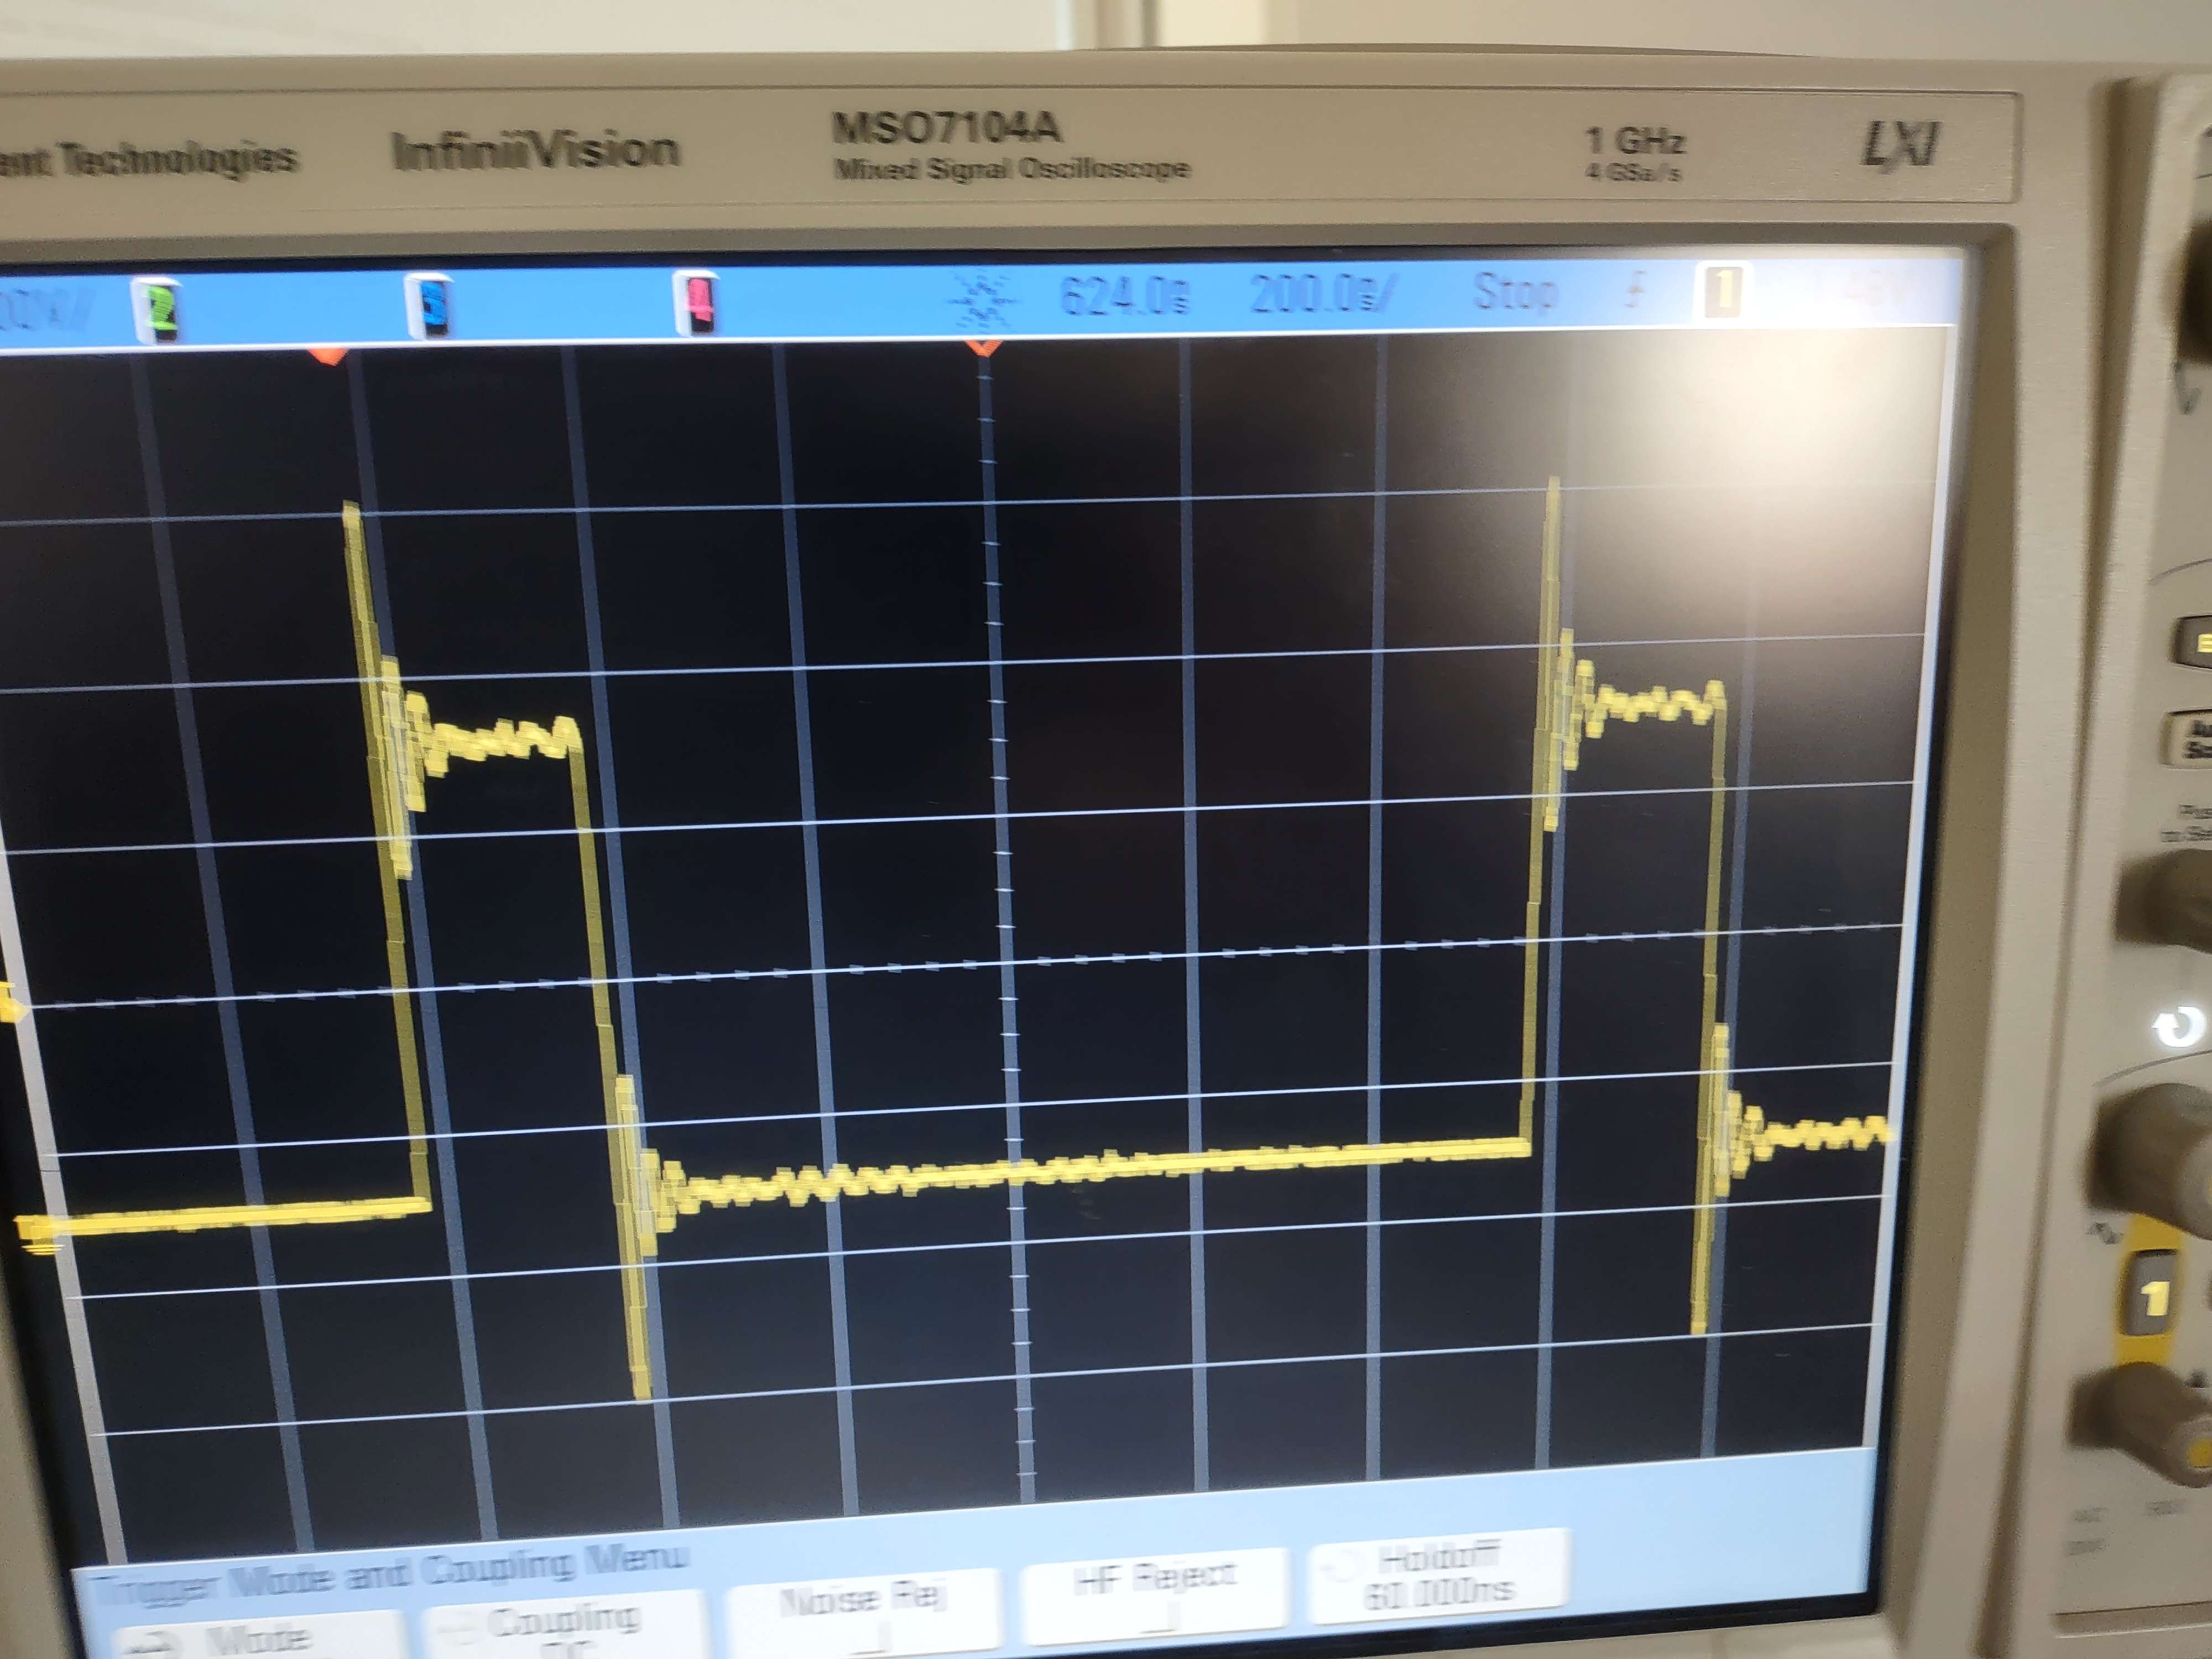
\includegraphics[width=\textwidth]{text/PraktickaCast/img/trampolina.jpg}
  \end{center}
  \label{Semisemafor-zvonek}
  \caption{Zarušená komunikace s ledkami}
\end{figure}

Tento problém jsem vyřešil doplněním feritu do cesty řídícího signálu, abych utlumil vyšší harmonické složky.

Kvůli servisním zákrokům a konstrukci krytu jsem navíc přidal i další dvě kontaktní plošky pod USB konektor pro možnost přehrání firmwaru bez nutnosti vyjmutí desky.
Výsledné schéma viz \ref{Semisemafor-sch-v2}

\section{Mechanické stavba}
Jedním z podstatných požadavků byla jistá úroveň krytí proti vodě, aby se zařízení dalo používat i za deště.
To nutně neznamená úplnou vodotěsnost, dá se totiž předpokládat, že zařízení bude používáno v poloze, kdy je powerbanka dole a Semisemafor nahoře.
Stačí tedy zajistit těsnost proti stékající vodě jen v jednom směru.

Navíc se během testování objevil ještě požadavek na zpětnou vazbu tlačítka v podobě jeho kliknutí. 
Uživatel totiž musí vědět, že tlačítko skutečně stiskl, na což je mechanická odezva samotného tlačítka ideální.

Po několika iteracích jsem obdržel výsledný vzhled (viz obrázek \ref{Semisemafor-box-render})
\begin{figure}[!h]
  \begin{center}
    \includegraphics[width=0.7\textwidth]{text/PraktickaCast/img/Semisemafor-BOX-render.png}
  \end{center}
  \label{Semisemafor-box-render}
  \caption{Vzhled Semisemaforu}
\end{figure}

Jako technologii výroby jsem zvolil obyčejný FDM 3D tisk.
Původně jsem chtěl použít materiál ASA pro jeho UV odolnost, ale ukázalo se, že jsem nebyl schopen navrhnout mechaniku tak, aby byl výsledek dostatečně voděodolný a zároveň měla tlačítka uspokojivou zpětnou vazbu.
ASA bylo příliš tuhé a cvaknutí mikrospínače příliš utlumilo, aby jej uživatel zaznamenal.
Stejné výsledky jsem měl z PETG, PLA, ABS a několika dalšími materiály. Jediný materiál, u kterého jsem dosáhl uspokojivých výsledků, byl PP (polypropylene).

Problém tisku polypropylenu je jeho tepelná roztažnost, takže pokud se tiskne za běžných teplot má tendenci se při tisku kroutit, což značně zesložiťuje jeho tisk.
Jednou možností by bylo celý tisk provádět při teplotě přes \(120^\circ C\), kde začíná probíhat rekrystalizace a polypropylen se začíná výrazně smršťovat.
Tato možnost ale nese nutnost použití speciální tiskárny, která umožňuje tiskový prostor vytopit na tak vysokou teplotu, a proto byla zvolena méně spolehlivá ale jednodušší metoda.
Použitá metoda je založena na vícemateriálovém tisku, přičemž primární je užitečný tisknutý objekt z polypropylenu a druhý dobře tisknutelný materiál tvoří podpěry a přítlak.
Aby tak bylo možné vytisknout i tvar, který nemá vhodná místa pro umístění přítlaku, musí být opatřen technologickými výstupky, které se po tisku mohou odříznout.

Tiskový model byl tedy doplněn o další objekt zajišťující přítlak a~zároveň i~podpěry.
Výsledek je vidět na obrázku \ref{Semisemafor-box-pritlak}

\begin{figure}[!h]
  \centering
  \includegraphics[width=0.9\textwidth]{text/PraktickaCast/img/Semisemafor-BOX-pritlak.png}
  \label{Semisemafor-box-pritlak}
  \caption{Soustava modelů pro tisk}
\end{figure}

Aby nebylo nutné pouzdro tisknout na více dílů, byla zvolena možnost zatiskávání DPS během tisku.
Pokaždé, když tisk dospěl do správného bodu, pozastavil se, aby bylo možné vložit elektroniku a následně pokračoval.

Kromě elektroniky bylo stejným postupem umisťováno i průhledové "sklíčko".
Aby bylo možné zachovat odolnost proti vodě, bylo toto "sklíčko" také z polypropylenu, aby se během tisku přivařilo k okolní hmotě a vytvořilo tak vodotěsný spoj.

Protože je DPS semaforu oboustranně osazena, byl při zatiskávání ještě jeden problém.
Buď by se totiž DPS vložila zarovnaná s aktuální tiskovou vrstvou plochou substrátu.
To by však znamenalo, že by tisková hlava mohla narazit do nějaké z vystupujících součástek.
Nebo tisknout od horního bodu nejvyšší součástky, což by ale znamenalo, že by elektronika nebyla pevně uchycena.
Tento problém byl vyřešen vložkou, která se před zatištěním přilepí na spodní stranu DPS a srovná ji do roviny.
Vložka navíc umožnila mít dodatečné kontaktní plošky z druhé strany USB, protože bez ní by se tyto plošky vyzkratovali o stínění USB konektoru.
Za tímto účelem byla také deska vyrobena v tloušťce 0.8mm, aby byly tyto dodatečné plošky lépe kryty. 
DPC opatřena vložkou je vidět na obrázku \ref{Semisemafor-vlozka}

\begin{figure}[!h]
  \centering
  \includegraphics[width=0.6\textwidth]{text/PraktickaCast/img/Semisemafor-vlozka.png}
  \label{Semisemafor-vlozka}
  \caption{DPS Semisemaforu opatřena vložkou}
\end{figure}

\begin{figure}[!h]
  \centering
  \includegraphics[width=0.8\textwidth]{text/PraktickaCast/img/Real-Semisemafor.jpg}
  \label{Semisemafor-real}
  \caption{Reálný kus Semisemaforu}
\end{figure}


Aby bylo tlačítko dostatečně měkké, mělo dostatečně silnou odezvu a zároveň bylo odolné vůči vodě.
Zvolil jsem tenkou membránu ze které vede šoupátko k tlačítku.
Při stisku membrány je tak pomocí šoupátka stisknuto i tlačítko.
Zároveň aby nebylo nutné mačkat přímo na místo kde je uchyceno šoupátko a aby se zabránilo možnému sklouznutí šoupátka z tlačítka.
Zesílil jsem střed membrány, takže se z membrány stal takový hmatník po obvodu uchycený k tělu Semisemaforu, jak je vidět na obr \ref{Semisemafor-rez-tlacitky}

\begin{figure}[!h]
  \centering
  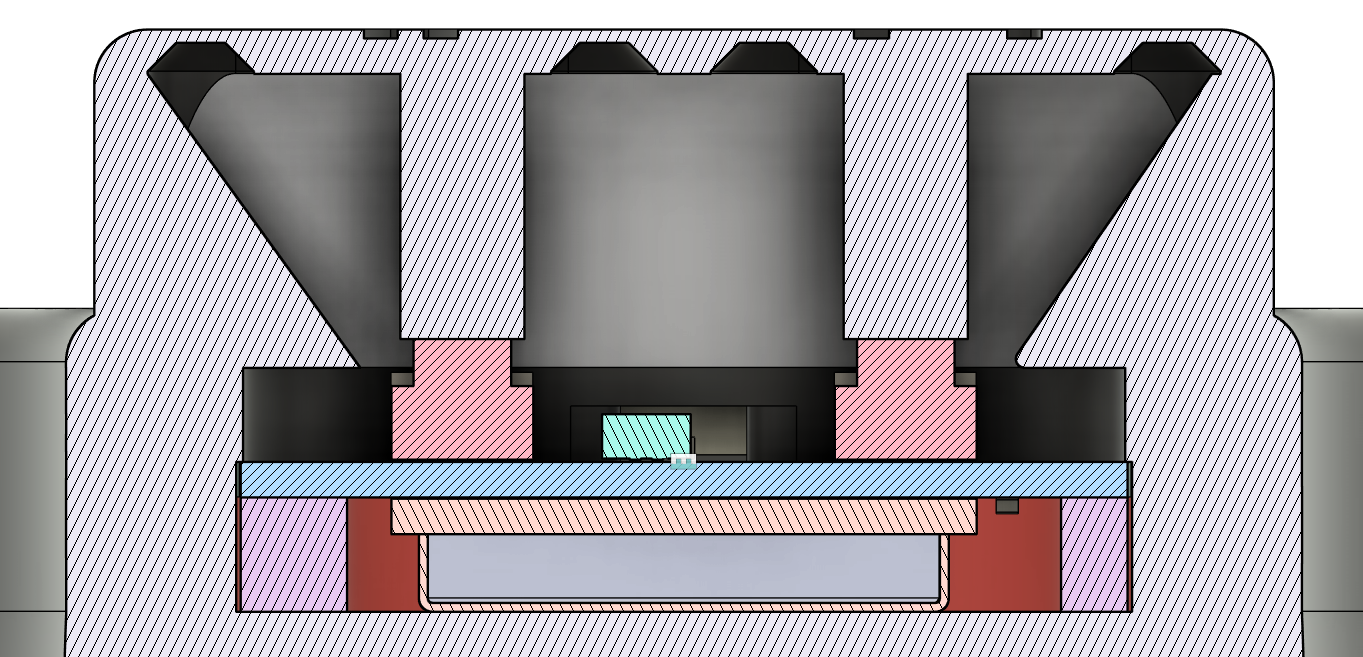
\includegraphics[width=0.8\textwidth]{text/PraktickaCast/img/RezSemaforem.png}
  \label{Semisemafor-rez-tlacitky}
  \caption{Řez tlačítky}
\end{figure}